% Reference: http://ctan.math.utah.edu/ctan/tex-archive/macros/latex/contrib/exam/examdoc.pdf
% https://www.sharelatex.com/learn/Typing_exams_in_LaTeX

% To create exam without answers, remove the answers arg from the command below
\documentclass[answers, addpoints, 12pt]{exam}
% \documentclass[addpoints, 12pt]{exam}
\usepackage[utf8]{inputenc}

\usepackage[margin=.75in]{geometry}

\usepackage{times}
\usepackage{amsmath,amsfonts,amssymb}
\usepackage[protrusion=true,expansion=true]{microtype}

\usepackage[shortlabels]{enumitem}
\usepackage{adjustbox}
\usepackage{booktabs}
\usepackage{caption}
\usepackage{fancyvrb}
\usepackage{floatrow}
\usepackage{graphicx}
\usepackage{listings}
\usepackage{listings}
\usepackage{multicol}
\usepackage{multicol}
\usepackage{subcaption}
\usepackage{verbatim}
\usepackage{wrapfig}
\usepackage{xcolor}

% Table float box with bottom caption, box width adjusted to content
\newfloatcommand{capbtabbox}{table}[][0.6\FBwidth]

\CorrectChoiceEmphasis{\color{red}}

\setlength{\emergencystretch}{3em}
\setlength{\parindent}{0em}
\setlength{\parskip}{1em}

\setlength{\columnsep}{.5cm}
\setlength{\columnseprule}{1pt}
\def\columnseprulecolor{\color{black}}

% If you need an image, stick it in the ./figs folder
\graphicspath{{./figs/}}

% Use \code{stuff} to make 'stuff' appear as code. Only useful for short
% amounts of code.
\newcommand{\code}[1]{\texttt{#1}}

\pointpoints{Pt}{Pts}

\title{Data 8 Final \color{red}{Solutions}}
% \title{Data 8 Final}
\author{Summer 2017}
\date{}

\newcommand{\class}{Data 8}
\newcommand{\term}{Summer 2017}
\newcommand{\examnum}{\color{red}{Final Solutions} }
% \newcommand{\examnum}{Final}
\newcommand{\examdate}{8/11/2017}
\newcommand{\timelimit}{170 Minutes}

\pagestyle{head}
\firstpageheader{}{}{}
\runningheader{\class}{\examnum\ - Page \thepage\ of \numpages}{\examdate}
\runningheadrule


\begin{document}

\maketitle

\makebox[\textwidth]{First Name:\enspace\hrulefill}
\vspace{0.1cm}

\makebox[\textwidth]{Last Name:\enspace\hrulefill}
\vspace{0.1cm}

\makebox[\textwidth]{Email:\enspace\hrulefill \code{@berkeley.edu}}
\vspace{0.1cm}

\makebox[\textwidth]{Student ID:\enspace\hrulefill}
\vspace{0.1cm}

\makebox[\textwidth]{GSI:\enspace\hrulefill}
\vspace{0.1cm}

\makebox[\textwidth]{Name of person to your left:\enspace\hrulefill}
\vspace{0.1cm}

\makebox[\textwidth]{Name of person to your right:\enspace\hrulefill}
\vspace{0.1cm}

\makebox[\textwidth]{\emph{All the work on this exam is my own.}
\textbf{(please sign)}: \enspace\hrulefill}
\vspace{0.1cm}

\begin{center}
\fbox{\fbox{
\parbox{6in}{
{\Large \textbf{Instructions:}}
\begin{itemize}
\item This exam contains \numpages\ pages (including this cover page) and
  \numquestions\ questions.
\item This exam must be completed in the given \textbf{2 hour, 50 minute} time
period.
\item You may use two handwritten (two-sided) cheat sheets and the two official
  study guides provided with this exam.
\item Work quickly through each question. There are a total of \numpoints\
  points on this exam.
\end{itemize}
}
}}
\end{center}

\newpage

\begin{center}
\vspace*{\stretch{1}}
This page is intentionally left blank, but feel free to use it as scratch
paper.
\vspace*{\stretch{1}}
\end{center}

\newpage

\begin{questions}

%!TEX root = ../final.tex
\question The \code{happy} table from Gallup World Poll data describes the
happiness score ratings of 157 countries. It contains the number of people (in
thousands) that gave each happiness rating (0 is worst, 10 is best) for each
country.

\begin{verbatim}
Country | Rating | Count
Denmark | 0      | 3.4
Denmark | 1      | 4.5
...     | ...    | ...
Denmark | 10     | 16.9
Iceland | 0      | 2.1
Iceland | 1      | 4.1
... (1510 rows omitted)
\end{verbatim}

Complete the Python expressions below to compute each result. The last line of
each answer should evaluate to the result requested. \textbf{You may not use
more lines than the ones provided.}

\begin{parts}

\part[2] The total number of people surveyed in the data, in thousands.

\begin{verbatim}
np.sum(_________________________________________________________)
\end{verbatim}

\begin{solution}
\begin{verbatim}
  np.sum(happy.column('Count'))
\end{verbatim}
\end{solution}

\part[3] A table containing the same columns as \code{happy} with the countries
in descending order by the number of people in that country who gave a rating
of 10. (All ratings in the table are integers.)

\begin{verbatim}
happy.__________________________________________________________
\end{verbatim}

\begin{solution}
\begin{verbatim}
happy.where('Rating', 10).sort('Count', descending=True)
\end{verbatim}
\end{solution}

\part[3] A table containing two columns: the countries and the total amount of
people surveyed for each country in thousands.
\begin{verbatim}
happy._________________________________________________________
\end{verbatim}

\begin{solution}
\begin{verbatim}
happy.drop('Rating').group('Country', np.sum)
\end{verbatim}
\end{solution}

\part[3] The average happiness rating of Denmark. (The answer is not simply 5.
Remember to account for the rating counts.)
\begin{verbatim}
d = ____________________________________________________________

sum(________________ * __________________) / sum(______________)
\end{verbatim}

\begin{solution}
\begin{verbatim}
d = happy.where('Country', 'Denmark')
sum(d.column(1) * d.column(2)) / sum(d.column(2))
\end{verbatim}
\end{solution}

\part[6] A table containing the average happiness rating for each country.
Assume you have a table called \code{totals} that contains the total
people surveyed for each country:

\begin{verbatim}
Country | Total
Denmark | 41.4
Iceland | 38.9
... (155 rows omitted)
\end{verbatim}

\begin{verbatim}
def helper(row):
    total = totals.____________________________________________

    return _________________ * ________________ / _____________

(happy.with_column('score', ___________________________________)
      .select('Country', 'score')
      .group('Country', np.sum))
\end{verbatim}

\begin{solution}
\begin{verbatim}
def helper(row):
    total = totals.where('Country', row.item(0)).column(1).item(0)
    return row.item(1) * row.item(2) / total

(happy.with_column('score', happy.apply(helper))
      .select('Country', 'score')
      .group('Country', np.sum))
\end{verbatim}
\end{solution}

\end{parts}


\newpage

%!TEX root = ../final.tex
% This question is basically ripped off from fa16 midterm
\question This question uses the following histogram of the number of gallons
of fuel consumed by different ships on the same trip.

\begin{figure}[h!]
  \centering
  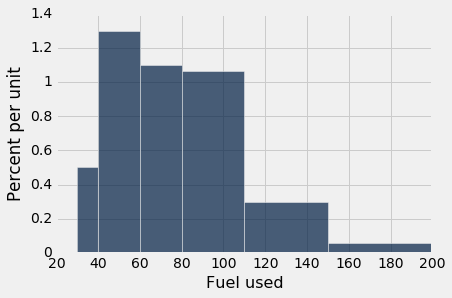
\includegraphics[height=5cm]{figs/fuel_bins.png}
  \label{fig:fuelbins}
\end{figure}

The heights of the bars (in percent per gallon of fuel) are:

\begin{center}
\begin{tabular}{ r || c | c | c | c | c | c }
 bin & [30, 40) & [40, 60) & [60, 80)
    & [80, 110) & [110, 150) & [150, 200) \\
 \hline
 height & 0.5 & 1.3 & 1.1 & 1.07 & ? & 0.06 \\
\end{tabular}
\end{center}

\begin{parts}
  \part[3] Find the missing bin height in percent per gallon of fuel. You may
  leave your answer as an expression. If it is not possible to find the height,
  explain why.

  \begin{solutionorbox}[1in]
  The areas of the bars must sum to 100 percent, so:
  \begin{align*}
    \frac{100 - 10(0.5) - 20(1.3) - 20(1.1) - 30(1.07) - 50(0.06)}{40} \approx
    0.296
  \end{align*}
  \end{solutionorbox}

  \part[3] Without any extra information, which bin has the most ships?

  \begin{oneparcheckboxes}
    \choice [40, 60)
    \choice [60, 80)
    \choice [80, 110)
    \choice Can't determine without additional information.
  \end{oneparcheckboxes}

  Justify your choice. If you picked the last choice, state the extra
  information you need.

  \begin{solutionorbox}[.7in]
  The [40, 60) bar has an area of: $ 20 * 1.3 = 26\% $.
  The [60, 80) bar has an area of: $ 20 * 1.1 = 22\% $.
  The [80, 110) bar has an area of: $ 30 * 1.07 = 30.21\% $.

  So, the [80, 110) bin has more ships regardless of how many ships there are total.
  \end{solutionorbox}

  \part[4] Suppose we merge the [30, 40) and [40, 60) bin together to create a
  single bin for [30, 60). What is the new height of [30, 60) bin (in percent
  per gallon)? You may leave your answer as an expression. If you need more
  information, state the information you need.

  \begin{solutionorbox}[2in]
  The [30, 40) bin has an area of: $ 10(0.5) = 5\% $. The [40, 60) bin has an area
  of $ 20(1.3) = 26\% $.

  The total area is then $ 31\% $. Dividing by the total width of the new bin
  we have a height of: $ 31 / (30) \approx 1.03 $.

  Note that you didn't need to know the number of ships in the [30, 40) bin to
  solve this problem!
  \end{solutionorbox}
\end{parts}


\newpage

%!TEX root = ../final.tex
\question A jar contains 100 jelly beans of four different colors - orange,
green, blue, and purple - in equal amounts. \textbf{In this question, if you
select the Other choice, you must state the correct expression in the space
provided.}

\begin{parts}
  \part[2] Suppose Sam only likes green jelly beans. He picks five beans at
  random without replacement from the jar. What is the chance he gets all green
  beans?

  \begin{multicols}{2}
  \begin{checkboxes}
    \correctchoice $ \frac{25}{100} \cdot \frac{24}{99} \cdot \frac{23}{98}
      \cdot \frac{22}{97} \cdot \frac{21}{96} $
    \choice $ \left( \frac{25}{100} \right)^5 $
    \choice $ \frac{25}{100} \cdot \frac{24}{100} \cdot \frac{23}{100} \cdot
      \frac{22}{100} \cdot \frac{21}{100} $
    \choice Other
  \end{checkboxes}
  \columnbreak
  If Other selected, write correct expression:
  \end{multicols}

  \part[3] Suppose he replaces the five previous beans and picks another five,
  this time with replacement. What is the chance he gets at least one green
  bean?

  \begin{multicols}{2}
  \begin{checkboxes}
    \choice $ 1 - \left( \frac{25}{100} \right)^5 $
    \choice $ 1 - \frac{25}{100} \cdot \frac{24}{100} \cdot \frac{23}{100}
      \cdot \frac{22}{100} \cdot \frac{21}{100} $
    \correctchoice $ 1 - \left(\frac{75}{100} \right)^5 $
    \choice Other
  \end{checkboxes}
  \columnbreak
  If Other selected, write correct expression:
  \end{multicols}

  \part[3] If Sam puts the beans back in the jar and then draws four beans
  without replacement, what is the chance that all four beans are different
  colors?

  \begin{multicols}{2}
  \begin{checkboxes}
    \choice $ \frac{25}{100} \cdot \frac{24}{99} \cdot \frac{23}{98} \cdot
      \frac{22}{97} $
    \choice $ 1 - \frac{25}{100} \cdot \frac{24}{99} \cdot \frac{23}{98} \cdot
      \frac{22}{97} $
    \choice $ \frac{25}{100} \cdot \frac{25}{99} \cdot \frac{25}{98} \cdot
      \frac{25}{97} $
    \correctchoice Other
  \end{checkboxes}
  \columnbreak
  If Other selected, write correct expression:
  \end{multicols}

  \begin{solution}

  \[ \frac{100}{100} \cdot \frac{75}{99} \cdot
     \frac{50}{98} \cdot \frac{25}{97} \]

  \end{solution}

  \part[4] Sam receives a gift jar of 400 jellybeans that has 50 orange, 50
  green, 150 blue, and 150 purple jellybeans. He's confused because he thinks
  the jar should have around the same proportion of each color, so he runs a
  hypothesis test.

  Null hypothesis: Each jellybean color has equal probability of
  appearing.

  Alternative: The jellybean colors appear with some other distribution.

  He selects the total variation distance as his test statistic.

  \begin{multicols}{2}
    Draw a rough sketch of the empirical distribution of the test statistic
    under the null hypothesis. You must:

    \begin{enumerate}
      \item Include the origin (0, 0) in your plot.
      \item Mark the observed value of the test statistic as a vertical line.
      \item Shade in the area corresponding to the P-value.
    \end{enumerate}

    Don't worry about x/y labels or whether you shaded in exactly the right
    amount of area.

    \columnbreak

    \begin{solutionorbox}[2in]
      TODO(sam): Add plot.
    \end{solutionorbox}
  \end{multicols}
\end{parts}


\newpage

%!TEX root = ../final.tex
\question Researchers collected data on the number of times students have
stepped on a UC Berkeley seal in the past year and students’ GPAs. A
scatterplot of GPA on number of steps (left), as well as the table \code{seal}
(middle) and its corresponding statistics (right), is displayed below. You may
assume that statistics in that table are good approximations to their
corresponding population parameters.

\begin{figure}[h!]
\begin{floatrow}
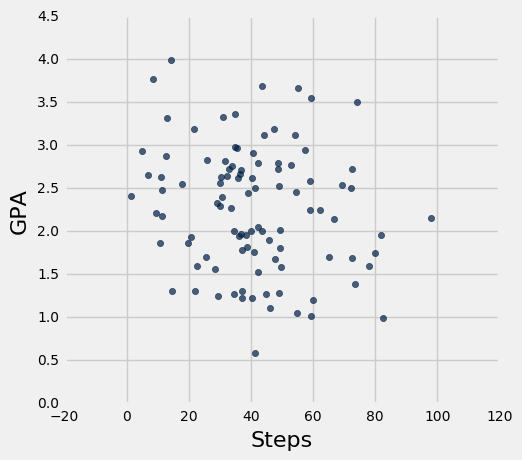
\includegraphics[width=0.18\textwidth]{figs/steps_and_gpa.png}
% \ffigbox{%
%   \rule{3cm}{3cm}%
% }{%
%   \caption{A figure}%
% }
\capbtabbox{%
  \begin{tabular}{|c|c|c|} \hline
  Student ID  & Steps   &  GPA \\ \hline
  25789012    &   65    &  2.86 \\ \hline
  38973744    &   39    &  3.76 \\ \hline
  31402938    &   96    &  3.12 \\ \hline
  \end{tabular}

  \code{... (97 rows omitted)}
}{}
\capbtabbox{%
  \begin{tabular}{|c|c|c|} \hline
  Statistic & Steps & GPA \\ \hline
  Mean      & 50    & 2.5 \\ \hline
  Std Dev   & 20    & 1.5 \\ \hline
  \end{tabular}
}{}
\end{floatrow}
\end{figure}

\begin{parts}

\part[4] Researchers want to create a confidence interval for the true slope of
the regression line predicting GPA given the number of steps on the seal.
Complete the code below so that the last line outputs a 90\% confidence
interval.

You may use the \code{slope(table, x\_label, y\_label)} function defined in
class which takes in a table, the label/index for the x-values, and the
label/index for the y-values, in that order. It returns the slope in original
units of the regression line predicting y given x.

\begin{verbatim}
slopes = make_array()
for i in np.arange(5000):

    resample = ___________________________________________________

    bootstrapped_slope = _________________________________________

    slopes = __________________ (slopes, _______________________ )

[percentile(________, slopes), percentile(________, slopes)]
\end{verbatim}

\begin{solution}
\begin{verbatim}
slopes = make_array()
for i in np.arange(5000):
    resample = seal.sample()
    bootstrapped_slope = slope(resample, "Steps", "GPA")
    slopes = np.append(slopes, bootstrapped_slope)

print(percentile(5, slopes), percentile(95, slopes))
\end{verbatim}
\end{solution}

\part[12] Assume the code above was implemented correctly and researchers
generate an interval of $(-0.25, 0.12)$ for the population regression slope.
Evaluate whether each statement is true or false and \textbf{briefly} justify
your answer.

\begin{subparts}
  \subpart Because the interval contains 0, for a p-value cutoff of
    5\% we fail to reject the null hypothesis that the slope of the population
    regression line is 0.

    \begin{oneparcheckboxes}
      \correctchoice True
      \choice False
    \end{oneparcheckboxes}

    \begin{solutionorbox}[0.8in]
      True. The confidence interval fails to reject this null hypothesis at a
      cutoff of 10\%, which means we would also fail to reject the null at a
      cutoff of 5\% (which gives a wider interval).
    \end{solutionorbox}

  \subpart If we rerun the code in part (a) 100 times, we expect that around 90
    of the intervals will contain the true population slope.

    \begin{oneparcheckboxes}
      \choice True
      \correctchoice False
    \end{oneparcheckboxes}

    \begin{solutionorbox}[0.8in]
      False. We aren't getting a new sample from the population, so if we reran
      the code in part (a) we would get approximately the same interval every
      time.
    \end{solutionorbox}

  \subpart The population regression slope falls within this interval about
    90\% of the time.

    \begin{oneparcheckboxes}
      \choice True
      \correctchoice False
    \end{oneparcheckboxes}

    \begin{solutionorbox}[0.8in]
      False. The population regression slope either falls within this
      interval or it doesn't.
    \end{solutionorbox}

  \subpart If we instead try to predict number of steps using GPA, we will
    still get roughly the same confidence interval endpoints.

    \begin{oneparcheckboxes}
      \choice True
      \correctchoice False
    \end{oneparcheckboxes}

    \begin{solutionorbox}[0.8in]
      False. Although the interval will likely contain 0, the units of the
      interval will be different so the endpoints will also be different.
    \end{solutionorbox}
\end{subparts}

\part[3] Suppose researchers are now interested in the average number of times
students have stepped on the UC Berkeley seal in the past year. What sample
size do they need to create a 95\% confidence interval such that the interval
width is 4 or less? If you need more information to solve this problem, state
what information you need.

\begin{solutionorbox}[1in]
The interval width must be 4 or less and there are 4 standard deviations in a
95\% confidence interval, so the standard deviation of the sample distribution
must be 1 or less. Using the sample standard deviation as an approximation for
the population standard deviation and applying the CLT, we get:

\begin{align*}
  \frac{20}{\sqrt{n}} &\leq 1 \\
  n &\geq 400
\end{align*}
\end{solutionorbox}

\checkboxchar{$\Box$}
\part[5] Using the data from \code{seal}, researchers create a 95\%
bootstrap confidence interval for the average number of times students have
stepped on a UC Berkeley seal in the past year. Which of the following
statements is/are true about this interval? Select all that apply.
\begin{checkboxes}
  \choice If researchers draw another sample and computed a second confidence
  interval, it will always overlap with the first interval.
  \choice If researchers increase their sample size from 100 to 1000, they will
  always get a smaller bootstrap confidence interval.
  \choice If the researchers increase their bootstrap resample size from 100 to
  1000, they will always get a confidence interval they can use to conduct a
  valid hypothesis test.
  \choice If the researchers increase their bootstrap repetitions from 5000 to
  10000, they can expect their confidence interval to be narrower.
  \correctchoice If the researchers resampled without replacement, the
  resulting interval will always have a width of 0.
\end{checkboxes}

\begin{solution}
  Choice 1 is false. We are not guaranteed that the intervals will overlap
  since we could get a sample that looks completely different from our first
  one.

  Choice 2 is false. We are not guaranteed that the new interval will be
  smaller, although it is highly likely.

  Choice 3 is false. We must resample the same number of items as the original
  sample for our confidence interval to be valid.

  Choice 4 is false. Increasing the bootstrap repetitions makes the empirical
  distribution of the test statistic smoother but does not significantly change
  the boundaries of the confidence interval.

  Choice 5 is true. If we resample without replacement, we will get the same
  resampled slope every time.
\end{solution}

\part[4] Which of the following statements are true about the confidence
interval created in part (a) and the confidence interval in part (d)? Select
all that apply.
\begin{checkboxes}
  \correctchoice Neither interval is guaranteed to contain the parameter it is trying to estimate.
  \choice The interval in part (d) will be wider because it has a higher
  confidence level.
  \choice The two intervals used different resample sizes.
  \choice The interval estimating the population regression slope can be used
  to test a null hypothesis, but the one estimating average steps on the seal
  cannot.
\end{checkboxes}

\begin{solution}
  Choice 1 is true. We are not guaranteed that either interval will contain
  the parameter.

  Choice 2 is false. The interval in (d) will be wider because it has
  different units, not because of its confidence level.

  Choice 3 is false. We must resample the same number of items as the original
  sample for both confidence intervals.

  Choice 4 is false. Both intervals can be used for hypothesis testing.
\end{solution}

\end{parts}


\newpage

%!TEX root = ../final.tex
\question Emma thinks that students can be classified either as a Berkeley
student or Stanford student by looking at each student's average number of
protests attended per semester and their average hours of sleep per night.

This scatter plot shows Emma's training set of three points for a
nearest-neighbor classifier.

\begin{figure}[h!]
  \centering
  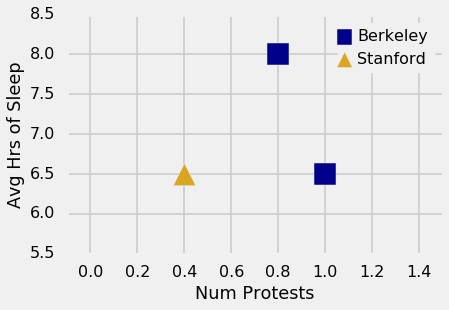
\includegraphics[scale=0.6]{class3}

  \textbf{Note that the axes are not on the same units.}
\end{figure}


\begin{parts}

\part[3] How would each unknown student be classified using a
1-nearest-neighbor classifier?

\begin{subparts}
  \subpart Student with 0.6 protests per semester and an average of 6.5 hours
  of sleep.

  \begin{oneparcheckboxes}
    \choice Berkeley
    \correctchoice Stanford
  \end{oneparcheckboxes}

  \subpart Student with 0.6 protests per semester and an average of 7.5 hours
  of sleep.

  \begin{oneparcheckboxes}
    \correctchoice Berkeley
    \choice Stanford
  \end{oneparcheckboxes}

  \subpart Student with 0 protests per semester and an average of 7.5 hours of
  sleep.

  \begin{oneparcheckboxes}
  \correctchoice Berkeley
  \choice Stanford
  \end{oneparcheckboxes}
\end{subparts}

\part[3] Draw the decision boundary for a 1-nearest neighbor classifier on the
scatterplot above.

\part[3] Suppose Emma's test set contains 100 examples all labeled Berkeley
that are distributed evenly throughout the area shown on the scatter plot
above. Which classifier will have a higher \textbf{test set} accuracy when
trained on her training set? Explain.

\begin{oneparcheckboxes}
  \choice A 1-nearest neighbor classifier
  \correctchoice A 3-nearest neighbor classifier
\end{oneparcheckboxes}

\begin{solutionorbox}[.9in]
  A 3-NN classifier will always predict Berkeley, which means it will have an
  prediction accuracy of 100\%.
\end{solutionorbox}

\part[3] Suppose Emma trains a 3-nearest neighbor classifier on her training
set. If we give the classifier a brand new point and it was classified
correctly, what is the probability that the new point was originally labeled
Stanford? Explain and show your work.

\begin{solutionorbox}[1in]
  Since a 3-NN classifier always classifies points as Berkeley, if the
  classifier was correct the point was originally labeled Berkeley with
  probability 1. This means that the probability that the point was originally
  labeled Stanford is 0.
\end{solutionorbox}

\end{parts}


\newpage

%!TEX root = ../final.tex
\question The \code{food} table contains the latitude and longitude of
restaurants in SF and their food safety rating (0 to 100, higher is better).

\begin{verbatim}
lat       | long        | score
37.791116 | -122.403816 | 98
37.786848 | -122.421547 | 100
37.792888 | -122.403135 | 70
... (6723 rows omitted)
\end{verbatim}

\begin{parts}

\part Sam tried to do some data analysis but didn't get very far. Here are some
variables he defined and how he defined them. The functions
\code{slope(table, x\_label, y\_label)} returns the slope in original units of
the regression line predicting y given x and \code{correlation(table, x\_label,
y\_label)} returns the correlation coefficient $r$ between the variables x and
y.

Write one line of Python code to compute each of the following.
\textbf{In your code, you may only use arithmetic operators, numbers, and the
variables that Sam defined below.}

\begin{verbatim}
name | code
a1   | slope(food, 'lat', 'score')
corr | correlation(food, 'lat', 'score')
m1   | np.mean(food.column('lat'))
m2   | np.mean(food.column('score'))
\end{verbatim}

\begin{subparts}
  \subpart[2] The correlation between score and latitude.

  \begin{verbatim}

____________________________________________________________
  \end{verbatim}

  \begin{solution}
  \begin{verbatim}
corr
  \end{verbatim}
  \end{solution}

  \subpart[3] The prediction for the score given a latitude of 750.

    \begin{verbatim}

____________________________________________________________
    \end{verbatim}

    \begin{solution}
    \begin{verbatim}
a1 * 750 + m2 - a1 * m1
    \end{verbatim}
    \end{solution}

  \subpart[3] The prediction for the latitude given a score of 0. (You don't
  need the next part of this question to solve this one.)

    \begin{verbatim}

____________________________________________________________
    \end{verbatim}

    \begin{solution}
    \begin{verbatim}
m1 - corr * corr / a1 * m2
    \end{verbatim}
    This question was taken out of the exam because you actually did, in fact,
    need part iv to solve this question.
    \end{solution}

  \subpart[3] The slope of the regression line predicting latitude given the
    score in original units.

    \begin{verbatim}

____________________________________________________________
    \end{verbatim}

    \begin{solution}
    \begin{verbatim}
corr * corr / a1
    \end{verbatim}
    \end{solution}
\end{subparts}

\newpage

\part[5] The \code{food} table is repeated here for your convenience.

\begin{verbatim}
lat       | long        | score
37.791116 | -122.403816 | 98
37.786848 | -122.421547 | 100
37.792888 | -122.403135 | 70
... (6723 rows omitted)
\end{verbatim}

Recall that the regression line is the line that minimizes the mean squared
error between the predictions and the actual values. For example, to find the
regression line that uses latitude to predict score we want to choose the slope
and intercept for the line:

\[ \text{predicted score} = slope \cdot lat + intercept \]

So that $ mean((\text{actual score} - \text{predicted score})^2) $ is as small
as possible.

We can use the \code{minimize} function to find this slope and intercept for
us. In particular, in lecture we defined a function
\code{mse(slope, intercept)} that returns the mean squared error given a
choice of slope and intercept. Then, \code{minimize(mse)} returned the slope
and intercept of the regression line.

What if we wanted to use both latitude and longitude to make a prediction? We
can do this by minimizing the mean squared error between the prediction line

\[ \text{predicted score} = slope_1 \cdot lat +
   slope_2 \cdot long + intercept \]

And the actual score. This is
also known by the term \emph{multiple linear regression}.

Fill in the the blanks for \code{multiple\_mse} so that
\code{minimize(multiple\_mse)} will return the three parameters for linear
regression using both latitude and longitude to predict score.

\begin{verbatim}

def multiple_mse(______________________________________________):

    lat = ______________________________________________________

    long = _____________________________________________________

    score = ____________________________________________________

    return np.mean(

    ____________________________________________________________
    )

\end{verbatim}

\begin{solution}
\begin{verbatim}
def multiple_mse(slope1, slope2, intercept):
    lat = food.column('lat')
    long = food.column('long')
    score = food.column('score')

    return np.mean(
      (score - slope1 * lat - slope2 * long - intercept) ** 2
    )
\end{verbatim}
\end{solution}

\end{parts}


\newpage

%!TEX root = ../final.tex
\question Arvind is testing the effectiveness of a drug, Oskirol, on patients
who suffer from the worldwide Tree Syndrome epidemic. He randomly selects 50
patients from the Junior University Hospital, then randomly assigns half of the
patients to a treatment group and half to control. He gives the treatment group
the drug and doesn't do anything to the control group.

Afterward, Arvind calculates an overall wellness score from 0 to 100 for all
patients. He creates a 95\% bootstrap confidence interval for the difference in
the mean wellness scores between treatment and control groups: [11.1,
18.4].

Sam has some complaints about Arvind's methods. Evaluate whether Sam is right
in each scenario and justify your answer.

\begin{parts}
  \part[3] Sam states that since Arvind only selected patients from the Junior
  University Hospital, Arvind cannot infer any effect his treatment has
  on \textbf{all} patients with Tree Syndrome.

  \begin{oneparcheckboxes}
    \correctchoice Sam is correct
    \choice Sam is incorrect
  \end{oneparcheckboxes}

  \begin{solutionorbox}[0.9in]
    Sam is correct. If Arvind only drew patients from the Junior University
    Hospital, with no other information he can only infer the effect his
    treatment has on patients with Tree Syndrome at that hospital.
  \end{solutionorbox}

  \part[3] Sam finds out that the true probability distribution of wellness
  scores is highly skewed left. Because of this, he states that the bootstrap
  is an \textbf{inappropriate method} to use.

  \begin{oneparcheckboxes}
    \choice Sam is correct
    \correctchoice Sam is incorrect
  \end{oneparcheckboxes}

  \begin{solutionorbox}[0.9in]
    Sam is incorrect. According to the Central Limit Theorem, the distribution
    of the mean wellness scores is normally distributed even though the actual
    distribution of scores is not, so the conditions for bootstrapping are
    still met.
  \end{solutionorbox}

  \part[3] Arvind notices that 0 is not in the confidence interval, so he
  concludes that is it likely his drug \textbf{caused} his patients' wellness
  scores to increase. Sam points out that Arvind's conclusion is incorrect:
  this hypothesis test can only be used to establish association, not
  causation.

  \begin{oneparcheckboxes}
    \choice Sam is correct
    \correctchoice Sam is incorrect
  \end{oneparcheckboxes}

  \begin{solutionorbox}[0.9in]
    Sam is incorrect. Because this experiment was a randomized control
    experiment, if we reject the null we can establish causality.

    Note that Arvind can conclude that his drug likely caused wellness scores
    to increase compared to patients who didn't take anything at all. He can't
    say anything about the effectiveness of his drug compared to a placebo
    which means this experiment needs adjusting for actual medical purposes.
  \end{solutionorbox}

  \part[3] Sam points out that Arvind didn't give a placebo to the
  control group, so the control group's wellness scores were not as high as
  they would be with a placebo. Sam argues that Arvind's confidence interval
  endpoints are likely \textbf{lower} than they would be with the placebo.

  \begin{oneparcheckboxes}
    \choice Sam is correct
    \correctchoice Sam is incorrect
  \end{oneparcheckboxes}

  \begin{solutionorbox}[0.9in]
    Sam is incorrect. Since we expect a placebo to increase the wellness scores
    of the control group, Arvind's confidence interval endpoints are likely
    higher that the one he would have created if he gave a placebo to the
    control group.
  \end{solutionorbox}

\end{parts}


\end{questions}

\newpage

\begin{center}
\vspace*{\stretch{1}}
This page is intentionally left blank, but feel free to use it as scratch
paper.
\vspace*{\stretch{1}}
\end{center}

\newpage

\end{document}
